% In this chapter:
% - introduction of eppex
% -- design goals
% -- distinction from legacy phrase-extract tools
% - implementation details
% -- Murmur hash, boost pools, std c++11 hash tables, indexed storages, gzipped I/O

\chapter{Eppex}
\label{chap:eppex}

\setlength{\epigraphwidth}{1.0\textwidth}
\epigraph{Your program can always have a twice as much time to run, but not always have a~twice as much memory.}{--- RNDr. Rudolf Kryl, "Programming II" course}

\Eppex{} is phrase pairs extraction and scoring tool capable of obtaining approximate
frequency counts of extracted phrase pairs by using Lossy Counting algorithm
(thus the name \eppex{}, an acronym for \emph{epochal phrase pairs extraction}).
It is designed to be an alternative to standard phrase extraction and scoring tools that
are shipped with Moses, implementing most of the functionality of steps 5 and 6 of
\emph{train-model.perl} script.
\Eppex{} input and output interface is fully compatible with the replaced tools
and \eppex{} in fact is intended to be invoked from within the Moses training script itself
by adding a few specific parameters.

\Eppex{} differs from its core counterparts in one important aspect: during its runtime,
only physical memory is utilized, no temporary files are stored on disk as with \emph{extract}
and \emph{score} tools.
The goal is to make \eppex{} a faster alternative, aiming at environments with plenty of RAM.
Benchmarking of time/memory trade-offs was the fundamental part of this work and the results are
thoroughly examined in \Cref{chap:results}.

\Eppex{} memory demands may be limited by setting more restrictive support and error thresholds
for Lossy Counting, but aggressive pruning may lead to loss of phrase table quality --
experimentally evaluated trade-offs are also discussed in \Cref{chap:results}.

This chapter is fully devoted to technical aspects of implementation and it expects the reader
to be familiar with the basics of programming and the C++ programming language, including
a basic knowledge of Standard Template Library (STL).
Instructions on how to install \eppex{} on Linux-based operating system are given in
\Aref{chap:installation}, usage instructions are given in \Aref{chap:usage}.

\section{Design goals and philosophy}

% What and why is a target platform?
\Eppex{} is implemented as a command-line program and, as indicated above, it is written in C++.
From the development perspective, \eppex{} adheres to the philosophy of Moses, what is mainly
reflected by the selection of development platform and third party libraries:
\begin{enumerate}
  \item The primary development platform is Linux --
  \eppex{} has been developed and tested on desktop version of Ubuntu 12.04 LTS with GCC~4.6.3 and
  server version of Ubuntu 10.04 LTS with GCC~4.4.3 installed.\footnote{GCC stands for the GNU Compiler Collection: \url{http://gcc.gnu.org/}}
  \item \Eppex{} relies on Boost C++ library\footurl{http://www.boost.org/} -- it is used to provide
  some essential functionality, so \eppex{} cannot be compiled without access to some of Boost
  headers and packages.\footnote{See \Aref{chap:installation} for details.}
\end{enumerate}
Nevertheless, a considerable effort has been taken to make the implementation as cross-platform
compatible as possible.

% 64-bit or 32-bit?
\Eppex{} is intended to be run on 64-bit machines, but this is rather a matter of fact than
a requirement: to process a parallel corpus of reasonable size, \eppex{} will in typical
setting require much more memory than 32-bit environments can provide\footnote{In 32-bit
environment the virtual address space holds no more than $2^{32}$ addresses, so at maximum
4,294,967,296 bytes (4~GB) of memory are utilizable. Workarounds exist, but they might be
considered unfeasible nowadays, as 64-bit architecture is well established.} (see
\Sref{sec:eppex-memory-demands} for some experimentally established figures).
Therefore, although not tested, \eppex{} should run as smoothly on 32-bit machine as it runs
on 64-bit, but the amount of input data that it will manage to process will have to be rather
small for practical MT or aggressive pruning will have to be undertaken.

\section{Effective C++}

% Why C++?
C++ is a programming language that offers a wide range of optimization techniques to
tune up both the execution speed and memory requirements of a program.
Both aspects are important to us, but memory usage optimization is our primary concern,
since the execution speed, when compared to legacy tools, is implicitly boosted by
the Lossy Counting algorithm and the fact that we keep all temporary data in the computer
memory instead of disk.
Besides, as pointed out in epigraph on the beginning of this chapter, memory, unlike time,
is a limited resource.
In this section we present several universal rules and techniques for effective C++
programming, that we followed and applied during implementation of \emph{eppex}.

\subsection{Data alignment and structure packing}

The issue behind \emph{data alignment} is best explained using example
-- let us define a dummy structure \texttt{LossyCounterItem}:

\begin{verbatim}
struct LossyCounterItem {
  unsigned char maximum_error; // sizeof(unsigned char) == 1
  unsigned int frequency; // sizeof(unsigned int) == 4
  unsigned short item_id; // sizeof(unsigned short) == 2
};
\end{verbatim}

Given the definition above and with respect to the byte sizes of individual members,
one could expect that \texttt{sizeof(LossyCounterItem)} equals to 7, but this guess
will be wrong in most of the cases. The most likely result is 12.

This unexpected behavior stems from the fact that many machines require that
objects of a certain type are aligned on architecture-dependent boundaries,
for example integers are often allocated on word\footnote{\emph{Word} in computer
architecture terminology denotes a fixed-sized group of bits that are handled
as a unit by the instruction  set and/or hardware of the processor.} boundaries
\citep[Chapter 5]{stroustrup:cplusplus}.

The easiest way how to minimize effects of data alignment is to order members
by their size with the largest members first.
This way our \texttt{LossyCounterItem} structure can be shrunk to 8 bytes,
but still there will be one byte of blank padding at the end of the structure.
With some compilers this padding can be trimmed by setting on \emph{structure packing}
using \texttt{\#pragma} preprocessor directive, but doing this will slow data access
on most processors that read memory by words, because misaligned structures will span
multiple words and in consequence require more reads.

This being said, the best solution in terms of code portability and effectiveness
is to design data structures in such a way that all their members properly align:
this ensures their effective handling by processing unit without spurious memory padding.

\subsection{C-string vs. std::string}
\label{sec:strings}
% Why had we used C-string instead of std::string.

Unlike Java, C and C++ have no fundamental data type for strings, instead they have
to be stored as an array of \texttt{chars}.
Such string handling is obviously too low-level for most modern applications,
which are mainly about string processing, so STL creators came to help and designed
several \emph{string} classes that mimic behavior of ordinary data types
\citep[Chapter 11]{josuttis:stl}:
STL strings may be copied, assigned and compared like any other fundamental type,
without the programmer being worried about the internal memory allocations and deallocations.
Because both approaches are very often used side by side, there exists well-established
terminology to distinguish between them:
the arrays of characters are called \emph{C-like-strings} (or shortly \emph{C-strings}) and
STL string classes are just \emph{strings} (sometimes labeled \emph{std::string} after the
most commonly used class).

From the memory management standpoint it turns out, that any std::string
implementation will be more memory demanding than plain C-string.
This is expectable: the STL string class has to provide more flexible interface
and does all the internal memory management by itself.
Depending on particular implementation, it might store the size of the string,
store the capacity of allocated memory, do the reference counting and more
\citep[Item 15]{meyers:effectivestl}.
The reference counting feature seems to be useful for our phrase-counting problem,
but it would imply to rely on proprietary implementation that is not enforced by
standard, which is a bad design choice for any open-source software.

Therefore, whenever the memory footprint of strings storage is more important than
the convenience and flexibility of their handling, C-string is a better choice
than any STL string implementation.

\subsection{Objects unification}
\label{sec:objects-unification}

When processing large stream of items that have the property of being distinguishable
either as different or equal to each other, it is often efficient to keep only a single
copy of each \emph{unique} item in the program memory and use some type of lightweight
reference to this copy in all the parts of program that have to access it.
In the C++ literature, this well-known technique is called \emph{reference counting}
\citep[Item 29]{meyers:more-effective-cpp}, but as the description of implementation
details later reveals, we are not interested in the proper reference counting,
because the copies we store this way are never individually destroyed.
Therefore, we rather refer to this simpler version of reference counting as \emph{objects
unification}.

%For example, when counting $n$-grams in a text corpus, instead of keeping $n$ strings
%within each $n$-gram object, it might be more efficient to just keep $n$ references to
%unique, separately stored copies of such strings.\footnote{An observant reader may realize
%that the task of items counting itself implicitly requires objects unification. In fact,
%the example was deliberately picked to demonstrate that there are two aspects to objects
%unification: it is a procedure inherent to some tasks, such as items counting, but also
%a technique to achieve some memory savings in general.}

Obviously, objects unification is not applicable universally and, in general,
its efficiency depends on the following factors:
\begin{enumerate}
  \item The input redundancy of items -- the greater the redundancy, the greater
  the possible memory savings. If there are no redundant items, this technique is useless,
  because it is cheaper to just store the item without an additional reference to it.
  \item The processing redundancy of items -- the more the items have to be
  referenced within the program, the greater the possible memory savings.
  \item The ratio between average in-memory size of item and reference to it -- the greater
  the ratio, the more memory is saved by each reference.
  Clearly, this ratio has to be greater than one.
\end{enumerate}

Typically, a programmer cannot affect the first factor, but should carefully consider it.
For example, in case of words pulled from natural language corpus it is generally hard to
presume whether their unification in program memory will be efficient:
Zipf's law \citep[Chapter 1]{manning:stat-nlp} suggests that the efficiency of words unification
will largely depend on the overhead imposed by the referencing scheme and if the references are
too heavy, the memory spared thanks to the most frequent words can be easily depleted by
the massive amount of words occurring only once.

The second factor might be tricky to consider in programs with non-linear work flow,
for example when the amount of items within program scope depends on some external
factor (time of day etc.), but in case of streamline input processing this value is
most often linear with respect to the input size.

The third factor is the only one that is completely in hands of the programmer.
With C++ we have two basic options, how to reference an object:
\begin{enumerate}
  \item by using object's address within memory
  \item by using a numeric index that uniquely identifies an object within a large storage
  (either a random access container or an array).
\end{enumerate}

We may note that both options are fundamentally the same:
the pointer is basically a numeric index into the container of a maximum size (entire memory)
and the numeric index is just a pointer into restrained part of memory (container).
The pointer is easier to dereference, but comes in single size only -- the size of
\emph{processor unit word}, which on 64-bit architecture is 8~bytes long.
On the other hand, to dereference the numeric index, a corresponding container must be
accessed to determine the address of index start.
However, a numeric index data type can be adjusted to the size of domain of unified items,
if it is known in advance or can be assessed by some upper bound.
Being able to reference 4~billions of unique objects is enough in many situations and
in such cases only 4~bytes long integer type will suffice, reducing referencing overhead
to half of that of the pointer.

As a final note, we shall point out that objects unification comes with a cost of
additional processing overhead: especially insertion of new object is more time-consuming,
as every new object have to be first checked for an existing copy.
Clearly, the efficiency of this technique has to be considered from case to case.

\subsection{Simple segregated storage}
\label{sec:simple-segregated-storage}

Almost every non-trivial computer program uses dynamic memory allocation.
C++ provides two interfaces to ask for a new memory during program runtime:
one can either use legacy C API function \emph{malloc} or pure C++ API operator \emph{new}.
Both APIs have to provide means to satisfy any type of memory request -- and for any size.
Hence, usually the size of an allocated memory block (and any other bookkeeping information) is
kept in the memory chunk right before the block itself \citep[Item 10]{meyers:effective-cpp}.
This way, for the deallocation either via \emph{free} function or operator \emph{delete},
the memory allocator only needs the pointer to the memory block that should be deallocated.
It can easily determine, how much memory should be actually freed, by inspecting the
bookkeeping information.

The obvious overhead in memory consumption incurred by this approach is usually negligible,
but may become significant in situations, when a load of small-sized memory blocks is allocated.
To avoid the overhead in such situations, a frequently used approach is to allocate a big pool of
fixed-size memory blocks once a time and serve these blocks sequentially as new memory requests
come in, allocating a new pool whenever all memory blocks in existing pools are exhausted.
This technique is generally called \emph{memory pooling}, but when details of
memory pool allocation and deallocation matters, usually more specific names are used to
distinguish between various implementations --  a \emph{simple segregated storage} from Boost
library is an example of one such specific
implementation.\footurl{http://www.boost.org/doc/libs/1_54_0/libs/pool/doc/html/boost_pool/pool/pooling.html}

% Unions - in current version of Eppex they don't play significant role.

\subsection{Unordered sets}

The recent C++ standard,\footnote{ISO/IEC 14882:2011} marked as C++11, standardizes
a new type of containers, that were already part of almost every implementation of STL,
but due non-existing standardization they differ slightly in their interfaces across
various implementations.
The \emph{unordered associative containers} are well known to almost every programmer,
although usually they are referred to under a different name: \emph{hash tables}.

The C++11 standard defines four types of hash table containers that correspond to existing
binary-search-tree-based containers (with an \emph{unordered_} prefix):
\emph{unordered_set}, \emph{unordered_multiset}, \emph{unordered_map} and \emph{unordered_multimap}.
The key differences between hash tables and binary-search trees are:
\begin{itemize}
  \item Binary-search trees require the "less-than" comparison operator to be defined for stored items,
  whereas hash tables require the "equal-to" comparison operator and also a hash function to be
  defined for them.
  \item When iterating over a binary-search tree, the items are returned in the order provided by
  the "less-than" comparison operator, whereas the iteration over hash table returns the items in arbitrary
  order.
  \item Lookup, insertion and deletion operations with hash tables have (amortized) constant
  average cost per operation (one call to the hash function plus one or more equality comparisons),
  whereas with binary-search tree these operations have a cost dependent on the number of items
  in the tree ($N$): each operation requires $O\big(log_2(N)\big)$ comparisons.
\end{itemize}

In the real life applications hash tables often perform much better than binary-search
trees, although their worst case complexity is linear with respect to number of items
(the C++ standard requires that hash tables are implemented using
\emph{closed addressing}\footurl{http://en.wikipedia.org/wiki/Hash_tables\#Separate_chaining}).
The effectiveness of hash tables stands and falls with the hash function:
a good hash function has to be fast to compute and possess the quality of distributing
the data as evenly as possible over its output range.

\section{Implementation analysis and description}

During the program runtime, the input data are processed in order to establish frequency counts
necessary to compute phrase pair scores and print the complete phrase translation table.
This requires the phrase pairs to be extracted and kept in memory along with the estimated
frequency and maximum error for Lossy Counting -- essentially, a set of triples $(e, f, \Delta)$,
as described in \Cref{chap:lossy-counting}, is to be maintained.
These data account for most of the memory required during runtime, therefore their effective
representation in memory is mission-critical and was object of the major programming effort.

\subsection{Size of integer types}

Both frequency count and maximum error are plain unsigned integers, so at first it might seem
there is nothing that can be possibly done about their optimization.
However, it will be unwise to just declare them both as \texttt{unsigned int}.
First, the size of integer data types is implementation dependent.
Despite that \texttt{int} is typically 4 bytes long, this is not guaranteed \citep[Chapter 4.6]{stroustrup:cplusplus}.
Second, it is important to realize that by processing real life data we may never need as much
space as some integer types provide and saving even few bytes per item can lead to gigabytes
saved in total.

To ensure cross-platform compatibility, we base the definitions of estimated frequency count and
maximum error (and other crucial numeric types) on definitions of fixed-size integer types from
Boost.Integer library.\footurl{http://www.boost.org/doc/libs/1_53_0/libs/integer/doc/html/index.html}
For frequency counts we dedicate 4~bytes, a space capable of storing all unsigned values up to
$2^{32} \approx 4.3 \times 10^9$. This is definitely enough for our task as there is no
parallel corpus yet with billions of parallel sentences, therefore it is safe to expect no phrase
pair will occur billion times.
For maximum error values it is sufficient to dedicate 1~byte only (unsigned values up to 255).
A maximum error of any item during Lossy Counting is always less than the ID of current epoch and
from our initial experiments, we had learned that lossy counted phrase extraction with more than just
a few epochs leads to pruning that already hurts too much.

\subsection{Phrase pair structure}

% Types of objects stored:
% - words, phrases, alignments

In contrast to counters, a phrase pair is quite a complex structure: it consist of the source phrase,
the target phrase and also the information about alignment between particular words of both phrases.
Both source and target phrases can be further decomposed into sequence of words, while alignment
information can be further decomposed into sequence of pairs of alignment points.
What makes the design of effective in-memory representation of such a structure even more complicated,
is the necessity to account for the variable lengths of these components.
%a phrase pair can have the source phrase of length $S$, the target phrase of length $T$ and
%the alignment information of length $L$, such that $S \neq T \neq L$.
On the other hand, there is a natural limit to these lengths incurred by the maximum sentence length and,
in practice, even a more restrictive limits are usually enforced to secure the feasibility of the
extracted translation model.

From the perspective of effective implementation, it is useful to break the phrase pair
structure into three subcomponents -- words, phrases and alignments -- and analyze them
independently.

%Let us first analyze the properties of each of these components independently and then
%conclude with the description of how they can be fit together to build a phrase pair.

\subsubsection*{Words}

Words or, more generally, translation model factors, are technically string-like types.
In \Sref{sec:strings}, we had discussed the advantage of C-strings over STL strings when
it comes to memory requirements.
Later, in \Sref{sec:objects-unification} we mentioned an approach that aims to spare the
overall memory demands of a program by using lightweight references to the unique copies of
data in places where the full copy would otherwise be stored.
With both these options in mind, it is easy to come up with an idea to store all words as
C-strings in a separate storage and keep only pointers to them in each phrase structure.
The problem with this idea is that a pointer type in 64-bits environments occupies
8~bytes, a space that is simply excessive for representation of a single word (a lot of
words could be fit into 8 bytes directly).

Instead, as already suggested in \Sref{sec:objects-unification}, it is more effective to
use a numeric index as a reference.
Arguably, words from a natural language present the input factor with the largest possible
variability and, despite that it is impossible to count the number of words in any language,
a reasonable estimate for English mentions the order of hundreds of thousands.\footurl{http://en.wikipedia.org/wiki/Number_of_words_in_English}
Therefore, the \texttt{boost::uint32_t} data type from Boost.Integer library, capable
of holding more than 4.2~billions of values, should be sufficient as a numeric index data
type for any reasonable input factor.

During the lossy counted extraction, the end-of-epoch pruning can remove all the phrase
pairs that reference a certain word and, in such a case, the unique copy of this word could
be deleted from the memory. However, we decided to not implement such functionality.
Intuitively, it seems more viable to spare the processing time overhead incurred by
the detection and removal of such words than try to spare a bit of space, most likely to
be rather insignificant in the overall scope: the number of unique words can reach
a million or two, but the number of unique phrase pairs will reach hundreds of millions.

\subsubsection*{Phrases}

With the words referenced by numeric indexes, it is straight-forward to structure phrase
as a sequence of such indexes and this is in fact the solution we sticked to.

An alternative implementation could employ objects unification, but the positive effect
of this technique is doubtful on this level, because there are far more distinct phrase
forms than there are word forms.
As mentioned in \Sref{sec:significance-pruning}, a typical phrase table contains a lot
of 1-1-1 phrase pairs.\footnote{In our experiments, the amount of 1-1-1 phrase pairs
accounted for 27\% and 40\% of the phrase tables, see \Cref{chap:results}.}
The source and target phrases in such phrase pairs are not only diminishing the
efficiency of objects unification, as they occur only once, but the phrase pair as such
pose a very likely candidate for pruning.
In contrast to the pruning of words data as discussed earlier, the pruning of phrase
data can have a very significant impact on the program memory footprint.
With the phrase data stored in a unique copy, to remove this copy we would have to
verify that there remain no other references pointing to it and this would require
either some reference counting scheme (additional memory overhead) or a full scan over
the copies and the references (additional processing overhead).

\subsubsection*{Alignments}

% Properties of phrase pair alignment.
The phrase pair alignment marks words from source and target side that were aligned to
each other in the word alignment of the sentence from which the phrase pair was extracted.
The phrase extraction algorithm ensures that each extracted phrase pair is based on
at least one alignment pair.
However, because there is no dependency between word-alignments of sentences,
a particular phrase pair can be encountered with multiple distinct alignments and only
the most frequent one should be included in the phrase table.\footnote{This is what Moses \emph{phrase-extract} toolkit does.}
Consequently, during the extraction of phrase pairs, it is necessary to track all the
distinct alignments encountered for each phrase pair, as well as theirs frequency counts.

For the purpose of in-memory representation, we decided to treat the phrase pair alignments
similarly to words and to use the same strategy to store them, i.e. keep unique copies in
a separate storage referenced by numeric indexes.

The main motivation for such decision was the finding that phrase pair alignments tend to
have a Zipfian-like frequency distribution, as \Fref{fig:alignment-dist} illustrates.
To obtain the plot, we extracted all (41.3~M) of phrase pairs of lengths up to~7 from
the Czech-English part of Europarl v6 parallel corpus and for each alignment counted
the number of distinct phrase pairs it has been matched with.
The extracted data contained more than 506~K of unique alignments and the most frequent
alignment "\texttt{0-0 1-1}" has been matched with more than 1.5~M of phrase pairs.
The number of unique phrase pairs suggests that the numeric index has to span at least
3 bytes.
Interestingly, no phrase pair have been matched with more than 9~different alignments.

\begin{figure}[ht]
  % GNUPLOT: LaTeX picture with Postscript
\begingroup
  \makeatletter
  \providecommand\color[2][]{%
    \GenericError{(gnuplot) \space\space\space\@spaces}{%
      Package color not loaded in conjunction with
      terminal option `colourtext'%
    }{See the gnuplot documentation for explanation.%
    }{Either use 'blacktext' in gnuplot or load the package
      color.sty in LaTeX.}%
    \renewcommand\color[2][]{}%
  }%
  \providecommand\includegraphics[2][]{%
    \GenericError{(gnuplot) \space\space\space\@spaces}{%
      Package graphicx or graphics not loaded%
    }{See the gnuplot documentation for explanation.%
    }{The gnuplot epslatex terminal needs graphicx.sty or graphics.sty.}%
    \renewcommand\includegraphics[2][]{}%
  }%
  \providecommand\rotatebox[2]{#2}%
  \@ifundefined{ifGPcolor}{%
    \newif\ifGPcolor
    \GPcolorfalse
  }{}%
  \@ifundefined{ifGPblacktext}{%
    \newif\ifGPblacktext
    \GPblacktexttrue
  }{}%
  % define a \g@addto@macro without @ in the name:
  \let\gplgaddtomacro\g@addto@macro
  % define empty templates for all commands taking text:
  \gdef\gplbacktext{}%
  \gdef\gplfronttext{}%
  \makeatother
  \ifGPblacktext
    % no textcolor at all
    \def\colorrgb#1{}%
    \def\colorgray#1{}%
  \else
    % gray or color?
    \ifGPcolor
      \def\colorrgb#1{\color[rgb]{#1}}%
      \def\colorgray#1{\color[gray]{#1}}%
      \expandafter\def\csname LTw\endcsname{\color{white}}%
      \expandafter\def\csname LTb\endcsname{\color{black}}%
      \expandafter\def\csname LTa\endcsname{\color{black}}%
      \expandafter\def\csname LT0\endcsname{\color[rgb]{1,0,0}}%
      \expandafter\def\csname LT1\endcsname{\color[rgb]{0,1,0}}%
      \expandafter\def\csname LT2\endcsname{\color[rgb]{0,0,1}}%
      \expandafter\def\csname LT3\endcsname{\color[rgb]{1,0,1}}%
      \expandafter\def\csname LT4\endcsname{\color[rgb]{0,1,1}}%
      \expandafter\def\csname LT5\endcsname{\color[rgb]{1,1,0}}%
      \expandafter\def\csname LT6\endcsname{\color[rgb]{0,0,0}}%
      \expandafter\def\csname LT7\endcsname{\color[rgb]{1,0.3,0}}%
      \expandafter\def\csname LT8\endcsname{\color[rgb]{0.5,0.5,0.5}}%
    \else
      % gray
      \def\colorrgb#1{\color{black}}%
      \def\colorgray#1{\color[gray]{#1}}%
      \expandafter\def\csname LTw\endcsname{\color{white}}%
      \expandafter\def\csname LTb\endcsname{\color{black}}%
      \expandafter\def\csname LTa\endcsname{\color{black}}%
      \expandafter\def\csname LT0\endcsname{\color{black}}%
      \expandafter\def\csname LT1\endcsname{\color{black}}%
      \expandafter\def\csname LT2\endcsname{\color{black}}%
      \expandafter\def\csname LT3\endcsname{\color{black}}%
      \expandafter\def\csname LT4\endcsname{\color{black}}%
      \expandafter\def\csname LT5\endcsname{\color{black}}%
      \expandafter\def\csname LT6\endcsname{\color{black}}%
      \expandafter\def\csname LT7\endcsname{\color{black}}%
      \expandafter\def\csname LT8\endcsname{\color{black}}%
    \fi
  \fi
  \setlength{\unitlength}{0.0500bp}%
  \begin{picture}(7200.00,5040.00)%
    \gplgaddtomacro\gplbacktext{%
      \csname LTb\endcsname%
      \put(1342,856){\makebox(0,0)[r]{\strut{} 1}}%
      \put(1342,1359){\makebox(0,0)[r]{\strut{} 10}}%
      \put(1342,1862){\makebox(0,0)[r]{\strut{} 100}}%
      \put(1342,2366){\makebox(0,0)[r]{\strut{} 1000}}%
      \put(1342,2869){\makebox(0,0)[r]{\strut{} 10000}}%
      \put(1342,3372){\makebox(0,0)[r]{\strut{} 100000}}%
      \put(1342,3876){\makebox(0,0)[r]{\strut{} 1e+06}}%
      \put(1342,4379){\makebox(0,0)[r]{\strut{} 1e+07}}%
      \put(1729,484){\makebox(0,0){\strut{} 1}}%
      \put(2574,484){\makebox(0,0){\strut{} 10}}%
      \put(3420,484){\makebox(0,0){\strut{} 100}}%
      \put(4266,484){\makebox(0,0){\strut{} 1000}}%
      \put(5112,484){\makebox(0,0){\strut{} 10000}}%
      \put(5957,484){\makebox(0,0){\strut{} 100000}}%
      \put(6803,484){\makebox(0,0){\strut{} 1e+06}}%
      \put(176,2541){\rotatebox{-270}{\makebox(0,0){\strut{}Frequency of alignment}}}%
      \put(4138,154){\makebox(0,0){\strut{}Rank of alignment based on the frequency}}%
      \put(4138,4709){\makebox(0,0){\strut{}Alignment frequency vs. rank based on the frequency}}%
    }%
    \gplgaddtomacro\gplfronttext{%
    }%
    \gplbacktext
    \put(0,0){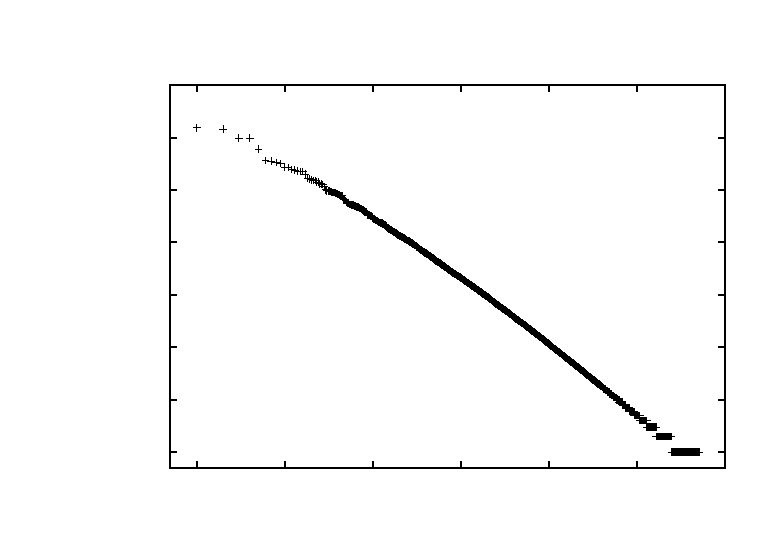
\includegraphics{alignments-distribution}}%
    \gplfronttext
  \end{picture}%
\endgroup

  \caption{
    A plot of phrase pair alignment frequency in a set of 41.3~M phrase pairs with
    506~K unique alignments extracted from the Czech-English part of Europarl v6 corpus.
    On the x axis is the rank of alignment based on the frequency, on y axis is the frequency.
  }
  \label{fig:alignment-dist}
\end{figure}

\subsubsection*{Phrase pairs}

The use of references to phrase pair alignments has one more advantage: all the main
components of a phrase pair can be stacked in a single array of 4-bytes-wide fields,
because the source and target phrases are just sequences of 4-byte-wide word indexes
and we empirically estimated 3~bytes of space to be enough for the numeric indexes
of the alignments.

Furthermore, the alignment frequency counter can also be represented with a 4~bytes
unsigned integer, because we demonstrated the same type to be capable of holding
the estimated frequency counts of phrase pairs in the Lossy Counter implementation.
In fact, a smaller data type will not suffice, as there might be a phrase pair with
only a single alignment.

Besides the components data, we also have to keep their dimensions,
to be able to tell where each component data starts and ends.
We already gave reasons, why to safely expect these values to be rather small and,
with a bit of static type casting, we can stack this information in the first
field of the array, so its layout will be as follows:
\begin{itemize}
  \item the first field contains a header-like structure with the count
    of distinct alignments $A$ (2~bytes),
    the source phrase length $S$ (1~byte) and the target phrase length $T$ (1~byte)
  \item the next $S$ fields contain word indexes of the source phrase
  \item the next $T$ fields contain word indexes of the target phrase
  \item the last $2 \times A$ fields contains a sequence of $A$ pairs with
    the alignment index and related frequency counter
\end{itemize}

Note that thanks to the fact that we store each alignment data separately, we do not
have to keep track of their lengths, because they are kept together with the unique copy.

The memory for the array is acquired via the operator \texttt{new}.
We experimented with an implementation using memory-pooled allocation,
but it had run terribly slow, presumably because of the frequent deallocation
of the phrase pair data.\footnote{A phrase pair data are deallocated not only
when a particular phrase pair is pruned, but also when a new alignment is
encountered and to accommodate it, the data has to be moved to a bigger array.}
Quite possibly, we did not employ the best memory pool implementation for such
purpose, so we keep this option in mind for the future work.

\subsection{Indexed storage}
% Indexed storage with memory pool

In the previous text, we did not provide any details about the actual implementation of
the storage that keeps the unique copies of words and alignments data.
Internally, we call this space an \emph{indexed storage}.

The implementation of \emph{indexed storage} employs three STL containers: one to keep
the actual data, one serving as a value-based lookup index and one serving as
a reference-based lookup index.

The actual string or sequence of alignment points is stored in a memory pool managed by
\texttt{boost::pool} class from the Boost Pool Library.\footurl{http://www.boost.org/doc/libs/1_54_0/libs/pool/doc/html/index.html}
This is the same implementation of memory pool that we had unsuccessfully tried to use
for allocation of memory for the phrase pair data.
Since no data is ever removed from \emph{indexed storage}, except for the whole storage
being purged as such, we did not encounter any performance issues in this case.

Pointers to each stored object are kept in a \texttt{vector} container: the position of
the pointer within the \texttt{vector} determines the value of the numeric index that
makes up the reference. This way, the referenced copy can be accessed in a constant time.

To be able to quickly determine, whether a particular string or alignment is present
in the storage, an additional index-like structure over the numeric indexes is maintained.
This structure is implemented with an \texttt{unordered_set} container, to provide
(amortized) constant lookup times.\footnote{The default \eppex{} compilation will, however,
use std::set instead of std::unordered_set, because the latter is still a rather recent
feature of C++.}
Although the container holds the numeric indexes, the value of hash function is calculated
over the data of an object to be checked. This way, whenever the object copy is already in
the \emph{indexed storage}, the correct numeric index can be immediately returned.

For the hash function, we chose the MurmurHash3 written by Austin Appleby and released as
public domain software.\footurl{http://code.google.com/p/smhasher/}
The MurmurHash3 is very robust and thus it is well suited for general hash-based lookup.

\subsection{Lossy Counter}

The Lossy Counter algorithm is implemented by a template class that is instantiated with
three parameters representing the different data types of triple $(e, f, \Delta)$.
The data structure $D$ is implemented via \texttt{unordered_map} with items $e$ being
the lookup keys and pairs $(f, \Delta)$ being the stored values (recall \Sref{sec:lossy-counting-definition}).

Since with every new alignment encountered for a particular phrase pair, its data has to
be updated, we had to tweak the implementation to allow for the constant keys of
\texttt{unordered_map} to be altered.

\subsection{Compressed I/O}

\Eppex{} can read/write directly from/to gzipped files, the same way legacy \emph{phrase-extract}
tools does.
This option allows to save a significant amount of disk space, as a typical phrase table will be
several times smaller when compressed.\footnote{In case of the phrase tables produced in our experiments
the compression ratio of the gzipped files varied between 14.0\% and 22.9\%.}
In addition, in environments when disks are under heavy load (shared computation servers are often
the case), compression may even speed up the whole I/O process.

Our implementation simply reuses the respective library shipped with Moses source code,
as it is cleanly designed and easy to include.
